\documentclass{article}
\usepackage[utf8]{inputenc}
\usepackage[margin=1in]{geometry}
\usepackage[titletoc,title]{appendix}
\usepackage{amsmath,amsfonts,amssymb,mathtools}
\usepackage{graphicx,float}
\usepackage[ruled,vlined]{algorithm2e}
\usepackage{algorithmic}
\usepackage{minted}
\setmintedinline{breaklines}
\usemintedstyle{solarized-dark}
\usepackage{biblatex}
\addbibresource{references.bib}
\usepackage{hyperref}
\usepackage{subcaption}
\usepackage{placeins}
\usepackage{flafter}

\title{AMATH 582 Final Project}
\author{Tyrone DeSilva}
\date{February 21, 2020}

\floatname{algorithm}{Procedure}
\renewcommand{\algorithmicrequire}{\textbf{Input:}}
\renewcommand{\algorithmicensure}{\textbf{Output:}}

\begin{document}
\maketitle

\begin{abstract}
\end{abstract}

\section{Introduction and Overview}

\section{Theoretical Background}

\section{Algorithm Implementation and Development}

\section{Computational Results}
\begin{figure}
    \centering
    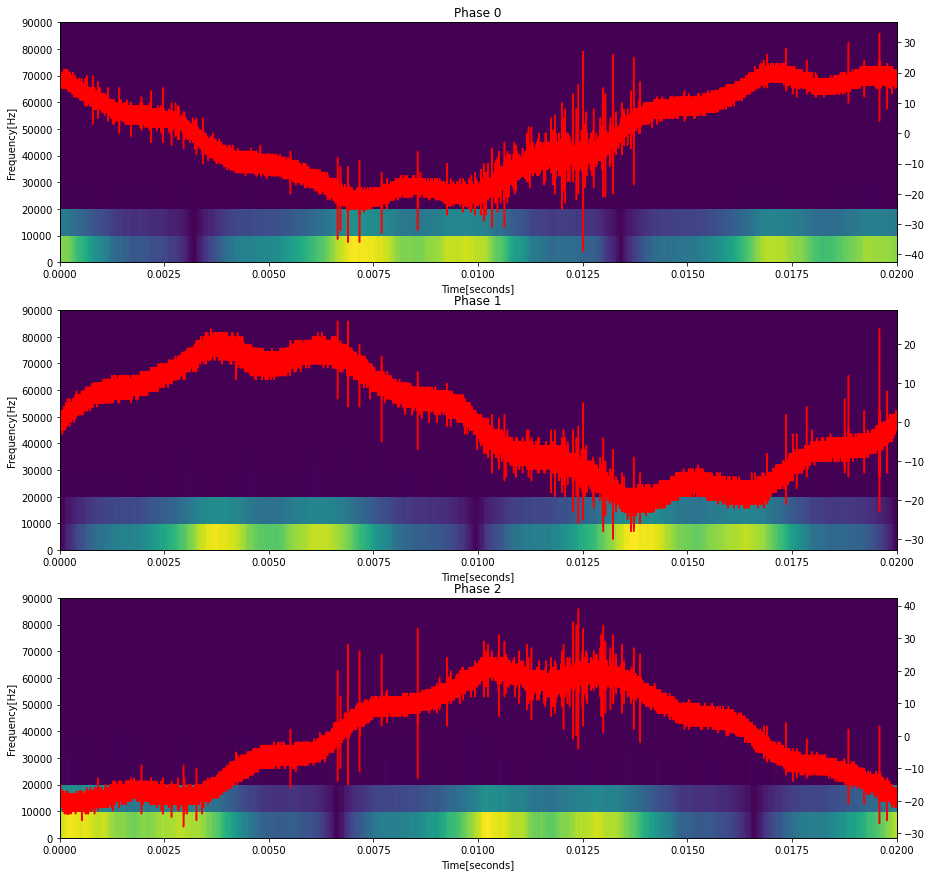
\includegraphics[width=0.8\linewidth]{stft.png}
    \caption{Periodograms for three phases along with original signals.}
    \label{fig:periodogram}
\end{figure}

\begin{figure}
    \centering
    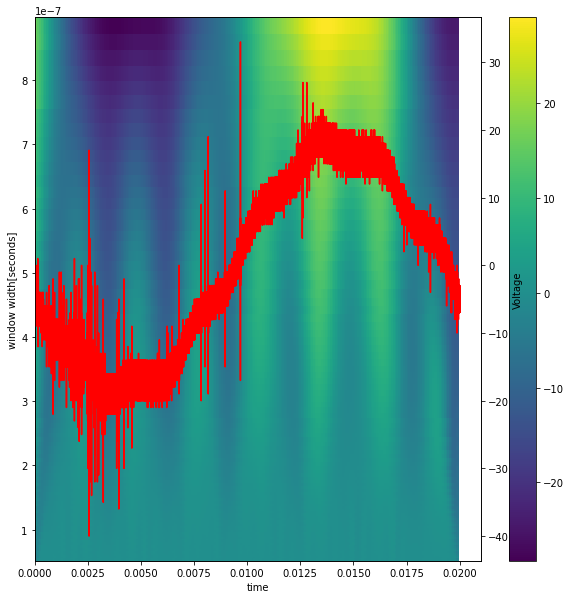
\includegraphics[width=0.6\linewidth]{cwt.png}
    \caption{Scalogram with original signal.}
    \label{fig:scalogram}
\end{figure}

\begin{figure}
    \centering
    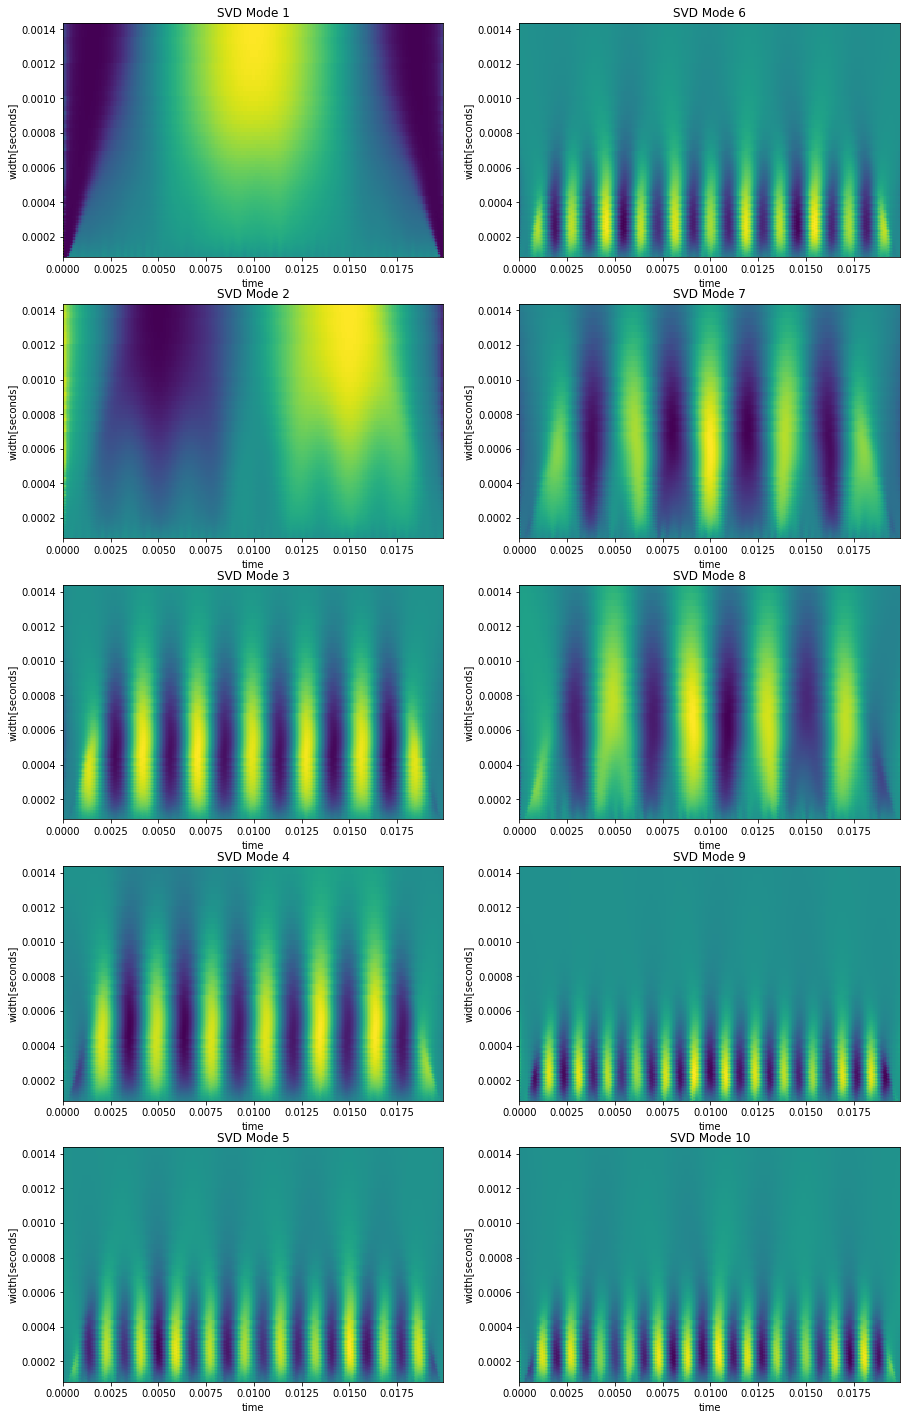
\includegraphics[width=0.8\linewidth]{pca_modes.png}
    \caption{PCA Modes}
    \label{fig:modes}
\end{figure}

\section{Summary and Conclusions}

\FloatBarrier
\printbibliography

\begin{appendices}
    \section{Python Functions}
        \label{sec:functions}
        \begin{itemize}
            \item Placeholder
        \end{itemize}
    \section{Python Code}
        \label{sec:code}
    \subsection{preprocess.py}
        \label{subsec:preprocess}
        \inputminted{python}{preprocess.py}
    \subsection{load.py}
        \label{subsec:load}
        \inputminted{python}{load.py}
    \subsection{pca\_modes.py}
        \label{subsec:pca_modes}
        \inputminted{python}{pca_modes.py}
    \subsection{pipeline.py}
        \label{subsec:pipeline}
        \inputminted{python}{pipeline.py}
    \subsection{plots.py}
        \label{subsec:plots}
        \inputminted{python}{plots.py}

\end{appendices}
\end{document}